\documentclass[12pt, a4paper]{report}

% Packages :

\usepackage[french]{babel}
\usepackage[utf8]{inputenc}
\usepackage[T1]{fontenc}
\usepackage[pdftex, pdfauthor={Bacomathiques}]{hyperref}
\usepackage{sectsty}
\usepackage[explicit]{titlesec}
\usepackage{xcolor}
\usepackage{amsmath}
\usepackage{amssymb}
\usepackage{amsthm}
\usepackage{fourier}
\usepackage{titlesec}
\usepackage{fancyhdr}
\usepackage{catchfilebetweentags}
\usepackage[french, capitalise, noabbrev]{cleveref}
\usepackage[fit, breakall]{truncate}
\usepackage[margin=3cm]{geometry}
\usepackage{tocloft}
\usepackage{tikz}
\usepackage{tocloft}
\usepackage{microtype}
\usepackage{listings}
\usepackage{tabularx}
\usepackage{calc}
\usepackage[export]{adjustbox}
\usepackage[most]{tcolorbox}
\usepackage{standalone}
\usepackage{xlop}
\usepackage{etoolbox}
\usepackage{environ}

\usetikzlibrary{arrows.meta}
\usetikzlibrary{trees}

% Paramètres :

\author{Bacomathiques}
\definecolor{graphe}{HTML}{93c9ff}
\setcounter{MaxMatrixCols}{12}
\setlength{\parindent}{0pt}
\setlength{\fboxsep}{0pt}
%\pdfsuppresswarningpagegroup=1

% Code :

\lstdefinestyle{style}{
	backgroundcolor=\color{white},
	commentstyle=\em\color[HTML]{999988},
	keywordstyle=\bfseries,
	identifierstyle=\normalfont,
	stringstyle=\color[rgb]{0.87, 0.07, 0.27},
	basicstyle=\ttfamily\color{black},
	breakatwhitespace=false,
	breaklines=true,
	captionpos=b,
	keepspaces=true,
	numbers=left,
	numbersep=5pt,
	showspaces=false,
	showstringspaces=false,
	showtabs=false,
	tabsize=2,
	numbers=none
}

\lstset{style=style}
\lstset{
	literate=
	{á}{{\'a}}1
	{à}{{\`a}}1
	{ã}{{\~a}}1
	{é}{{\'e}}1
	{ê}{{\^e}}1
	{í}{{\'i}}1
	{ó}{{\'o}}1
	{õ}{{\~o}}1
	{ú}{{\'u}}1
	{ü}{{\"u}}1
	{ç}{{\c{c}}}1
}

\lstset{
	framextopmargin=10pt,
	framexrightmargin=10pt,
	framexbottommargin=10pt,
	framexleftmargin=10pt,
	xleftmargin=10pt,
	xrightmargin=10pt,
}

% Couleurs :

\definecolor{title}{HTML}{912c21}
\definecolor{section}{HTML}{1c567d}
\definecolor{subsection}{HTML}{2980b9}

\definecolor{rule}{HTML}{c4c4c4}

\definecolor{formula}{HTML}{ebf3fb}
\definecolor{formula-left}{HTML}{3583d6}

\definecolor{tip}{HTML}{dcf3d8}
\definecolor{tip-left}{HTML}{26a65b}

\definecolor{demonstration}{HTML}{fff8de}
\definecolor{demonstration-left}{HTML}{f1c40f}

\definecolor{exercise}{HTML}{e0f2f1}
\definecolor{exercise-left}{HTML}{009688}

\definecolor{correction}{HTML}{e0f7fa}
\definecolor{correction-left}{HTML}{00bcd4}

\definecolor{toc}{HTML}{fceae9}
\definecolor{toc-left}{HTML}{e74c3c}
\definecolor{toc-dark}{HTML}{87281f}

% Titres :

\renewcommand{\thesection}{\Roman{section} - }
\renewcommand{\thesubsection}{\arabic{subsection}. }

\newcommand{\sectionstyle}{\normalfont\LARGE\bfseries\color{section}}
\titleformat{\section}{\sectionstyle}{\thesection #1}{0pt}{}
\titleformat{name=\section, numberless}{\sectionstyle}{#1}{0pt}{}

\newcommand{\subsectionstyle}{\normalfont\Large\bfseries\color{subsection}}
\titleformat{\subsection}{\subsectionstyle}{\thesubsection #1}{0pt}{}
\titleformat{name=\subsection, numberless}{\subsectionstyle}{#1}{0pt}{}

\titlelabel{\thetitle\ }

% Table des matières :

\addto\captionsfrench{\renewcommand\contentsname{}}
\renewcommand{\cftsecpagefont}{\color{toc-dark}}
\renewcommand{\cftsubsecpagefont}{\color{toc-dark}}
\renewcommand{\cftsecleader}{\cftdotfill{\cftdotsep}}
\renewcommand{\cftsecfont}{\bfseries}
\renewcommand{\cftsecpagefont}{\bfseries\color{toc-dark}}
\setlength{\cftbeforetoctitleskip}{0pt}
\setlength{\cftaftertoctitleskip}{0pt}
\setlength{\cftsecindent}{0pt}
\setlength{\cftsubsecindent}{20pt}
\setlength{\cftsubsecnumwidth}{20pt}

% Commandes :

\newcommand{\newpar}{\\[\medskipamount]}
\newcommand{\lesson}[3]{%
	\newcommand{\level}{#1}%
	\newcommand{\id}{#2}%
	\hypersetup{pdftitle={#3}}
	\begin{center}%
		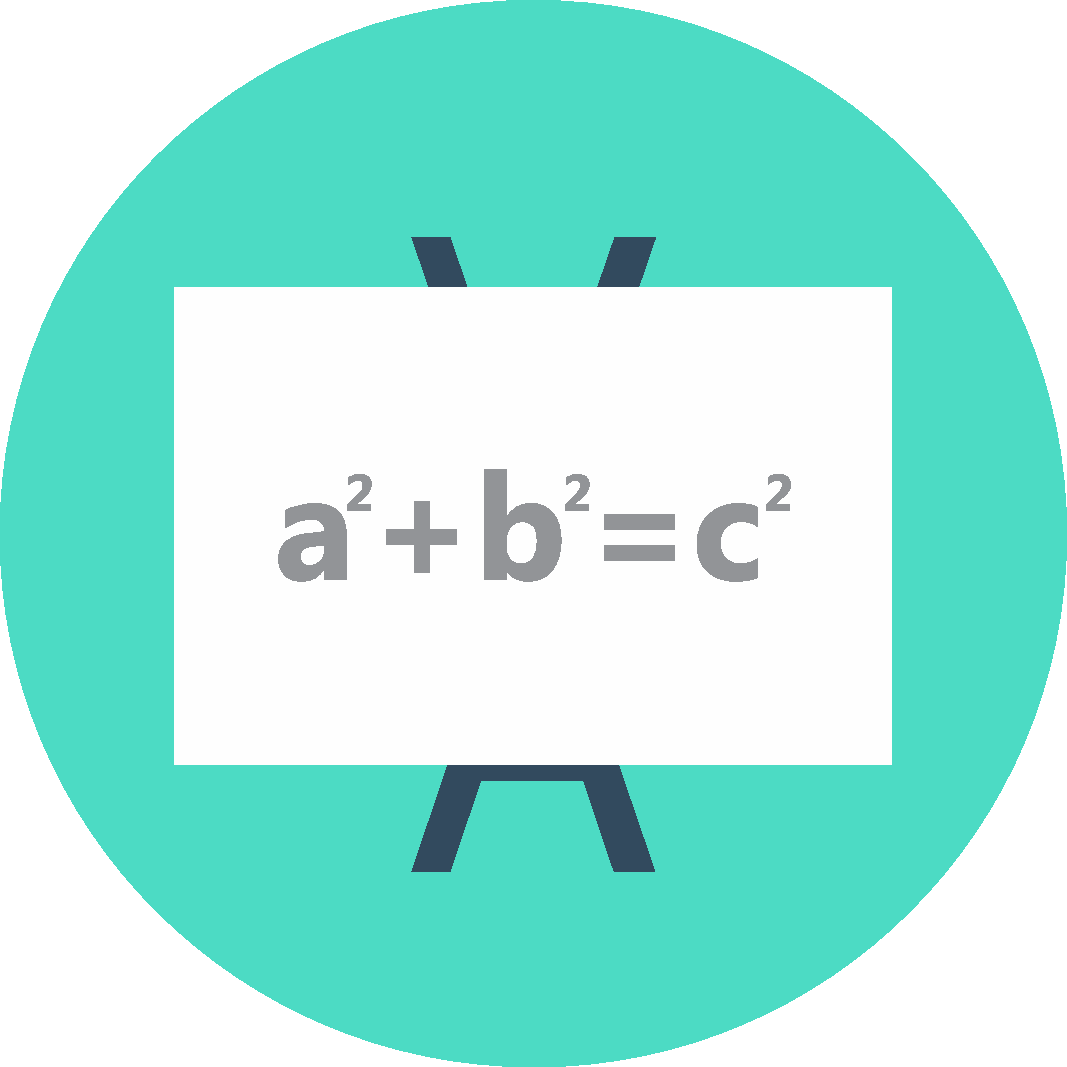
\includegraphics[width=150px]{\imagespath/bacomathiques}%
		
		\vspace{30pt}%
		{\Huge\color{title} #3}%
		
		\vspace{10pt}%
		{Bacomathiques --- \href{https://bacomathiqu.es/cours/#1/#2}{\color{section} https://bacomathiqu.es}}%
		
		\vspace{20pt}%
	\end{center}%
	\begin{toc}
		\tableofcontents%
	\end{toc}
	\thispagestyle{empty}%
	\newpage%
	\setcounter{page}{1}%
}
\newcommand{\imagespath}{../../images}
\newcommand{\lessonimagespath}{\imagespath/lessons/\level/\id/}
\newcommand{\includelatexpicture}[2][\textwidth - 100pt]{%
	\begin{center}%
		\resizebox{#1}{!}{%
			\input{\lessonimagespath#2}%
		}%
	\end{center}%
	\medskip%
}
\newcommand{\includeimage}[1]{%
	\begin{center}%
		\includegraphics{\lessonimagespath#1}%
	\end{center}%
	\medskip%
}
\newcommand{\includerepresentation}[1]{%
	\begin{center}%
		\setlength{\fboxrule}{0.5pt}%
		\href{https://www.geogebra.org/m/#1}{\includegraphics[width=\textwidth-1pt,fbox]{\lessonimagespath#1}}%
	\end{center}%
}
\newcommand{\floor}[1]{\lfloor #1 \rfloor}

\makeatletter
\newcommand\inputcontent{\@ifstar{\inputcontent@star}{\inputcontent@nostar}}
\newcommand{\inputcontent@star}[1]{%
	\ExecuteMetaData[#1]{content}%
}
\newcommand{\inputcontent@nostar}[1]{%
	\newpage%
	\inputcontent@star{#1}%
}
\makeatother

\let\oldsection\section
\renewcommand\section{\clearpage\oldsection}
\newcommand{\contentwidth}[1][medium]{}

% En-têtes :

\pagestyle{fancy}

\renewcommand{\sectionmark}[1]{\markboth{\thesection \ #1}{}}

\fancyhead[R]{\truncate{0.23\textwidth}{\color{title}\thepage}}
\fancyhead[L]{\truncate{0.73\textwidth}{\color{title}\leftmark}}
\fancyfoot[C]{\scriptsize \href{https://bacomathiqu.es/cours/\level/\id}{\texttt{bacomathiqu.es}}}

\makeatletter
\patchcmd{\f@nch@head}{\rlap}{\color{rule}\rlap}{}{}
\patchcmd{\headrule}{\hrule}{\color{rule}\hrule}{}{}
\makeatother

% Environnements :

\newenvironment{nosummary}{}{}
\newcommand{\tcolorboxtitle}[2]{\setlength{\fboxsep}{2.5pt}\hspace{-10pt}\colorbox{#1-left}{\hspace{8pt}\MakeUppercase{#2} \hspace{2pt} \includegraphics[height=0.8em]{\imagespath/bubbles/#1}\hspace{5pt}}}
\newcommand{\tcolorboxsubtitle}[2]{\ifstrempty{#2}{}{\textcolor{#1-left}{\large#2}\\[\medskipamount]}}
\tcbset{
	frame hidden,
	boxrule=0pt,
	boxsep=0pt,
	enlarge bottom by=8.5pt,
	enhanced jigsaw,
	boxed title style={sharp corners,boxrule=0pt,coltitle={white},titlerule=0pt},
	fonttitle=\fontsize{6pt}{6pt}\bfseries\boldmath,
	top=10pt,
	right=10pt,
	bottom=10pt,
	left=10pt,
	arc=0pt,
	outer arc=0pt,
}
\newtcolorbox{toc}[1][]{
	colback=toc,
	borderline west={3pt}{0pt}{toc-left},
	title=\tcolorboxtitle{toc}{Table des matières},
	colbacktitle=toc,
	before upper={\tcolorboxsubtitle{toc}{#1}}
}
\newtcolorbox{formula}[1][]{
	colback=formula,
	borderline west={3pt}{0pt}{formula-left},
	title=\tcolorboxtitle{formula}{À retenir},
	colbacktitle=formula,
	before upper={\tcolorboxsubtitle{formula}{#1}}
}
\newtcolorbox{tip}[1][]{
	colback=tip,
	borderline west={3pt}{0pt}{tip-left},
	title=\tcolorboxtitle{tip}{À lire},
	colbacktitle=tip,
	before upper={\tcolorboxsubtitle{tip}{#1}}
}
\newtcolorbox{demonstration}[1][]{
	colback=demonstration,
	borderline west={3pt}{0pt}{demonstration-left},
	title=\tcolorboxtitle{demonstration}{Démonstration},
	colbacktitle=demonstration,
	before upper={\tcolorboxsubtitle{demonstration}{#1}}
}

\NewEnviron{whitetabularx}[1]{%
	\renewcommand{\arraystretch}{2.5}
	\colorbox{white}{%
		\begin{tabularx}{\textwidth}{#1}%
			\BODY%
		\end{tabularx}%
	}%
}

% Longueurs :

\newlength{\espacetitreliste}
\setlength{\espacetitreliste}{-16pt}
\newcommand{\entretitreetliste}{\vspace{\espacetitreliste}}

\begin{document}
	%<*content>
	\lesson{terminale}{matrices-graphes}{Chapitre XV – Matrices et graphes (Maths expertes)}

	\section{Matrices}

	\subsection{Définition}

	\begin{formula}[Définition]
		Soient $m$ et $n$ deux entiers non nuls. Une \textbf{matrice réelle} $A$ de taille $m \times n$ est un tableau de réels tel que :
		\newpar
		$\displaystyle{A = \begin{pmatrix}a_{1,1} & a_{1,2} & \dots & a_{1,n} \\ a_{2,1} & a_{2,2} & \dots & a_{2,n} \\ \vdots & \vdots & \ddots & \vdots \\ a_{m,1} & a_{m,2} & \dots & a_{m,n}\end{pmatrix}}$
		\newpar
		Où $a_{1,1}$, $a_{1,2}$, $a_{2,1}$, ..., $a_{m,n}$ sont les \textbf{coefficients} de la matrice. L'ensemble des matrices à coefficients réels est noté $\mathcal{M}_{m,n}(\mathbb{R})$.
	\end{formula}

	Il serait également possible de prendre des matrices à coefficients entiers ou même complexes, mais nous nous limiterons ici au cas des matrices réelles.

	\begin{formula}[Types de matrices]
		Selon leur taille, on peut avoir différents types de matrices :
		\begin{itemize}
			\item Une matrice $1 \times n$ est une \textbf{matrice ligne de taille $n$}.
			\item Une matrice $m \times 1$ est une \textbf{matrice colonne de taille $m$}.
			\item Une matrice $n \times n$ est une \textbf{matrice carrée d'ordre $n$}. L'ensemble de ces matrices est noté $\mathcal{M}_n(\mathbb{R})$.
			\item Une matrice $1 \times 1$ est un \textbf{réel}.
			\item La matrice $m \times n$ dont tous les termes sont nuls est la \textbf{matrice nulle} et est notée $0_{\mathcal{M}_{m,n}(\mathbb{R})}$ (ou plus simplement $0_{m,n}$).
		\end{itemize}
	\end{formula}

	\subsection{Types de matrices carrées}

	\begin{formula}[Types de matrices carrées]
		Il existe différentes matrices carrées remarquables :
		\begin{itemize}
			\item Une matrice carrée dont tous les coefficients en dessous de la diagonale principale sont nuls est une \textbf{matrice triangulaire supérieure}.
			\item Une matrice triangulaire supérieure dont les coefficients sur la diagonale sont nuls est une \textbf{matrice triangulaire supérieure stricte}.
			\item Une matrice carrée dont tous les coefficients au-dessus de la diagonale principale sont nuls est une \textbf{matrice triangulaire inférieure}.
			\item Une matrice triangulaire inférieure dont les coefficients sur la diagonale sont nuls est une \textbf{matrice triangulaire inférieure stricte}.
			\item Une matrice carrée dont tous les coefficients qui ne sont pas sur la diagonale sont nuls est une \textbf{matrice diagonale}.
			\item Une matrice diagonale dont les coefficients sont égaux à $1$ est une \textbf{matrice identité}. Si la taille d'une telle matrice est $n$, alors on la note $I_n$.
		\end{itemize}
	\end{formula}

	\begin{tip}[Diagonale d'une matrice carrée]
		La diagonale d'une matrice carrée d'ordre $n$ représente l'ensemble des coefficients $a_{i,i}$ où $i$ varie de $1$ à $n$.
	\end{tip}

	\section{Opérations sur les matrices}

	\subsection{Somme}

	\begin{formula}[Somme de deux matrices]
		\contentwidth[big]
		Pour additionner deux matrices de même taille, il suffit d'additionner leurs coefficients deux-à-deux. Plus spécifiquement :
		\newpar
		$\displaystyle{\begin{pmatrix}a_{1,1} & a_{1,2} & \dots & a_{1,n} \\ a_{2,1} & a_{2,2} & \dots & a_{2,n} \\ \vdots & \vdots & \ddots & \vdots \\ a_{m,1} & a_{m,2} & \dots & a_{m,n}\end{pmatrix} + \begin{pmatrix}b_{1,1} & b_{1,2} & \dots & b_{1,n} \\ b_{2,1} & b_{2,2} & \dots & b_{2,n} \\ \vdots & \vdots & \ddots & \vdots \\ b_{m,1} & b_{m,2} & \dots & b_{m,n}\end{pmatrix}}$
		\newpar
		$\displaystyle{= \begin{pmatrix}a_{1,1} + b_{1,1} & a_{1,2} + b_{1,2} & \dots & a_{1,n} + b_{1,n} \\ a_{2,1} + b_{2,1} & a_{2,2} + b_{2,2} & \dots & a_{2,n} + b_{2,n} \\ \vdots & \vdots & \ddots & \vdots \\ a_{m,1} + b_{m,1} & a_{m,2} + b_{m,2} & \dots & a_{m,n} + b_{m,n}\end{pmatrix}}$
	\end{formula}

	\begin{tip}[Attention !]
		Il n'est possible d'additionner que deux matrices de même taille.
	\end{tip}

	\subsection{Produit}

	\begin{formula}[Multiplication d'une matrice par un réel]
		Soit $\lambda$ un réel. Le produit d'une matrice par $\lambda$ est la matrice de même taille dont les coefficients sont tous multipliés par $\lambda$. Plus spécifiquement :
		\newpar
		$\displaystyle{\lambda \times \begin{pmatrix}a_{1,1} & a_{1,2} & \dots & a_{1,n} \\ a_{2,1} & a_{2,2} & \dots & a_{2,n} \\ \vdots & \vdots & \ddots & \vdots \\ a_{m,1} & a_{m,2} & \dots & a_{m,n}\end{pmatrix} = \begin{pmatrix}\lambda \times a_{1,1} & \lambda \times a_{1,2} & \dots & \lambda \times a_{1,n} \\ \lambda \times a_{2,1} & \lambda \times a_{2,2} & \dots & \lambda \times a_{2,n} \\ \vdots & \vdots & \ddots & \vdots \\ \lambda \times a_{m,1} & \lambda \times a_{m,2} & \dots & \lambda \times a_{m,n}\end{pmatrix}}$
		\newpar
		Si $A$ est la matrice de gauche, on note $\lambda A$ la matrice de droite.
	\end{formula}

	\begin{tip}[Soustraction de deux matrices]
		Pour soustraire deux matrices $A$ et $B$, on additionne $A$ et $(-1)B$ i.e. $A - B = A + (-1)B$.
	\end{tip}

	\begin{formula}[Produit d'une matrice ligne et d'une matrice colonne]
		Soient $L = \begin{pmatrix}l_1 & ... & l_n\end{pmatrix}$ une matrice ligne de taille $n$ et $C = \begin{pmatrix}c_1 \\ \vdots \\ c_n\end{pmatrix}$ une matrice colonne de taille $n$.
		\newpar
		Le produit de ces deux matrices (noté $LC$) est le réel $LC = l_1 \times c_1 + \dots + l_n \times c_n$.
	\end{formula}

	Plus généralement, le produit matriciel ne se limite pas qu'à la multiplication d'une matrice ligne avec une matrice colonne.

	\begin{formula}[Produit de deux matrices]
		Soient $A$ une matrice de taille $m \times n$ et $B$ une matrice de taille $n \times p$ deux matrices. Le produit de ces deux matrices (notée $A \times B$ ou $AB$) est la matrice de taille $m \times p$ dont le coefficient à la position $(i; j)$ est égal au produit de la $i$-ième ligne de $A$ par la $j$-ième colonne de $B$. Plus spécifiquement, en notant $L_i$ la $i$-ème ligne de $A$ et $C_j$ la $j$-ième colonne de $B$ :
		\newpar
		$\displaystyle{AB = \begin{pmatrix}c_{1,1} & c_{1,2} & \dots & c_{1,p} \\ c_{2,1} & c_{2,2} & \dots & c_{2,p} \\ \vdots & \vdots & \ddots & \vdots \\ c_{m,1} & c_{m,2} & \dots & c_{m,p}\end{pmatrix}}$ où $c_{i,j} = L_i \times C_j$.
	\end{formula}

	\begin{tip}[Attention !]
		Le produit matriciel n'est pas commutatif ! Donc en général, $AB \neq BA$.
		\newpar
		De plus, il faut bien s'assurer que le nombre de lignes de $A$ est égal au nombre de colonnes de $B$.
	\end{tip}

	\begin{tip}
		Si $A$ et $B$ sont deux matrices diagonales de taille $n$. Leur produit est la matrice diagonale de même taille dont le coefficient à la position $(i; i)$ est le produit du coefficient de $A$ à la position $(i;i)$ par celui du coefficient de $B$ à la position $(i;i)$. Plus spécifiquement, en notant $A = (a_{i,j})$ et $B = (b_{i,j})$ :
		\newpar
		$\displaystyle{\begin{pmatrix}a_{1,1} & 0 & \dots & 0 \\ 0 & a_{2,2} & \dots & 0 \\ \vdots & \vdots & \ddots & \vdots \\ 0 & 0 & \dots & a_{n,n}\end{pmatrix} \times \begin{pmatrix}b_{1,1} & 0 & \dots & 0 \\ 0 & b_{2,2} & \dots & 0 \\ \vdots & \vdots & \ddots & \vdots \\ 0 & 0 & \dots & b_{n,n}\end{pmatrix}}$
		\newpar
		$\displaystyle{= \begin{pmatrix}a_{1,1} \times b_{1,1} & 0 & \dots & 0 \\ 0 & a_{2,2} \times b_{2,2} & \dots & 0 \\ \vdots & \vdots & \ddots & \vdots \\ 0 & 0 & \dots & a_{n,n} \times b_{n,n}\end{pmatrix}}$
		\newpar
		De plus, on a $AB = BA$.
	\end{tip}

	\begin{formula}[Propriétés du produit matriciel]
		Soient $A$, $B$ et $C$ trois matrices carrées d'ordre $n$. Alors :
		\begin{itemize}
			\item Le produit matriciel est \textbf{associatif} : $A(BC) = (AB)C$.
			\item Le produit matriciel est \textbf{distributif} : $A(B + C) = AB + AC$.
			\item $I_n$ est l'\textbf{unité} de $\mathcal{M}_{n}(\mathbb{R})$ : $AI_n = I_nA = A$.
			\item $0_n$ est le \textbf{zéro} de $\mathcal{M}_{n}(\mathbb{R})$ : $A0_n = 0_nA = 0_n$ et $A + 0_n = A$.
			\item Pour tout $\lambda \in \mathbb{R}$, $\lambda (AB) = (\lambda A)B = A(\lambda B)$.
		\end{itemize}
	\end{formula}

	\begin{tip}[Attention !]
		Si on a une égalité du type $A \times B = 0$, cela n'implique pas forcément que $A = 0$ ou $B = 0$ !
		\newpar
		De plus, si on a $AB = AC$, on n'a pas forcément $B = C$.
	\end{tip}

	Cela peut sembler logique, mais on signale tout de même que les priorités les opératoires sont ``les mêmes'' que dans les ensembles de nombres comme $\mathbb{R}$ ou $\mathbb{C}$ (la multiplication prime sur l'addition, etc...).

	\subsection{Inverse et déterminant}

	\begin{formula}[Inverse d'une matrice]
		Soit $A$ une matrice carrée d'ordre $n$. $A$ est dite inversible s'il existe une matrice $A^{-1}$ telle que $A \times A^{-1} = I_n$.
		\newpar
		Si cette matrice existe, elle est unique et s'appelle \textbf{inverse} de $A$. De plus, $A$ et $A^{-1}$ commutent.
	\end{formula}

	Le \textbf{déterminant} permet, entre autres, de calculer l'inverse d'une matrice (s'il existe). Nous nous limiterons ici au cas des matrices carrées d'ordre $2$, mais il est possible de le généraliser encore plus.

	\begin{formula}[Déterminant d'une matrice $2 \times 2$]
		Soit $\displaystyle{A = \begin{pmatrix} a & b \\ c & d \end{pmatrix}}$ une matrice carrée d'ordre $2$.
		\newpar
		Alors le déterminant de $A$ (noté $\det(A)$) est le réel $\det(A) = ad - bc$. De plus, $A$ est inversible si et seulement si $\det(A) \neq 0$.
	\end{formula}

	\begin{formula}[Inverse d'une matrice $2 \times 2$]
		Soit $\displaystyle{A = \begin{pmatrix} a & b \\ c & d \end{pmatrix}}$ une matrice carrée d'ordre $2$ dont le déterminant ne s'annule pas.
		\newpar
		Alors $\displaystyle{A^{-1} = \frac{1}{\det(A)} \begin{pmatrix} d & -b \\ -c & a \end{pmatrix}}$.
	\end{formula}

	\begin{tip}[Exemple]
		Calculons le produit de $\displaystyle{A = \begin{pmatrix}2 & 1 \\ 6 & 4\end{pmatrix}}$ par $\displaystyle{B = \begin{pmatrix}4 & -1 \\ -6 & 2\end{pmatrix}}$, et déduisons-en que $A$ est inversible sans utiliser la formule donnée précédemment.
		\newpar
		Le produit nous donnera une matrice carrée d'ordre $2$ car on multiplie deux matrices carrées d'ordre $2$ :
		\newpar
		$\displaystyle{\begin{pmatrix} 2 & 1 \\ 6 & 4 \end{pmatrix} \times \begin{pmatrix} 4 & -1 \\ -6 & 2\end{pmatrix} = \begin{pmatrix}8-6 & -2+2 \\ 24-24 & -6+8 \end{pmatrix} = \begin{pmatrix} 2 & 0 \\ 0 & 2 \end{pmatrix}}$
		\newpar
		Donc $A \times B = 2I_2$. Ainsi, $A$ est inversible et $A^{-1} = \frac{1}{2} B$.
	\end{tip}

	\subsection{Puissance}

	\begin{formula}[Puissance d'une matrice carrée]
		Soient $A$ une matrice carrée d'ordre $n$ et $i$ un entier naturel :
		\begin{itemize}
			\item Si $i \gt 0$, $\displaystyle{A^i = \underbrace{A \times \dots \times A}_{i \text{ fois}} = A^{i-1} \times A}$.
			\item Si $i = 0$, $A^i = A^0 = I_n$.
			\item Si $i \lt 0$, $\displaystyle{A^i = \underbrace{A^{-1} \times \dots \times A^{-1}}_{i \text{ fois}} = A^{i-1} \times A^{-1}}$.
		\end{itemize}
		De plus, pour tout entier naturel $j$, on a $A^i \times A^j = A^{i+j}$.
	\end{formula}

	\begin{tip}[Puissance d'une matrice diagonale]
		Si $A$ est une matrice diagonale, alors $A^i$ est la matrice de même taille où tous les termes de la diagonale sont mis à la puissance $i$ (cela vaut aussi si $i$ est négatif et que la diagonale ne comporte pas de $0$).
	\end{tip}

	\subsection{Transposition}

	\begin{formula}[Définition]
		Soit $A$ une matrice. La \textbf{matrice transposée} de $A$ (notée $^tA$) est la matrice dont la $i$-ième ligne correspond à la $i$-ième colonne de $A$.
	\end{formula}

	\begin{tip}[Exemple]
		Soient $\displaystyle{A = \begin{pmatrix} 2 & 5 & 9 \\ 3 & 6 & 10 \end{pmatrix}}$ et $\displaystyle{B = \begin{pmatrix} 0 & 1 & 1 \\ 2 & 3 & 5 \\ 8 & 13 & 21 \end{pmatrix}}$. Calculons $^tA$ et $^tB$.
		\newpar
		On a $\displaystyle{^tA = \begin{pmatrix} 2 & 3 \\ 5 & 6 \\ 9 & 10 \end{pmatrix}}$ et $\displaystyle{^tB = \begin{pmatrix} 0 & 2 & 8 \\ 1 & 3 & 13 \\ 1 & 5 & 21 \end{pmatrix}}$.
	\end{tip}

	\section{Applications}

	\subsection{Écriture matricielle d'un système d'équations linéaires}

	\begin{formula}[Lien entre système d'équations linéaires et matrices]
		Soient quatre réels $a$, $b$, $c$ et $d$ et soient deux réels $\alpha$ et $\beta$. Le système d'équations linéaires à deux inconnues $\displaystyle{(S) : \begin{cases}ax + by = \alpha \\ cx + dy = \beta\end{cases}}$ (d'inconnues $x$ et $y$) peut s'écrire matriciellement :
		\newpar
		$\displaystyle{(S) \iff \underbrace{\begin{pmatrix}a & b \\ c & d\end{pmatrix}}_{= \, A} \underbrace{\begin{pmatrix}x \\ y\end{pmatrix}}_{= \, X} = \underbrace{\begin{pmatrix}\alpha \\ \beta\end{pmatrix}}_{= \, B}}$
	\end{formula}

	\begin{formula}[Résolution du système $(S)$]
		Avec les notations ci-dessus, si $A$ est inversible (voir les paragraphes suivants) alors le système $(S)$ admet une unique solution $X = A^{-1}B$.
	\end{formula}

	\begin{tip}[Exemple]
		Cela peut sembler compliqué à appliquer, mais il n'en est rien !
		\newpar
		Par exemple, transformons le système $\displaystyle{(S) : \begin{cases}x + 2y = 1 \\ 2x + 5y = 4 \end{cases}}$ en une égalité de matrices :
		\newpar
		$\displaystyle{(S) \iff \begin{pmatrix}1 & 2 \\ 2 & 5\end{pmatrix} \begin{pmatrix}x \\ y\end{pmatrix} = \begin{pmatrix}1 \\ 4 \end{pmatrix}}$
		\newpar
		Or l'inverse de $\displaystyle{\begin{pmatrix}1 & 2 \\ 2 & 5\end{pmatrix}}$ est $\displaystyle{\begin{pmatrix}5 & -2 \\ -2 & 1\end{pmatrix}}$. D'où $\displaystyle{\begin{pmatrix}x \\ y\end{pmatrix} = \begin{pmatrix}5 & -2 \\ -2 & 1\end{pmatrix} \begin{pmatrix}1 \\ 4\end{pmatrix} = \begin{pmatrix}-3 \\ 2\end{pmatrix}}$.
		\newpar
		Or deux matrices sont égales si et seulement si leurs coefficients sont tous égaux. Donc on a $x = -3$ et $y = 2$.
	\end{tip}

	Nous avons travaillé ici avec un système de deux équations, mais il est tout à fait possible de généraliser cette méthode à plus de deux équations !

	\subsection{Suites de matrices colonnes}

	\begin{formula}
		Soit $(U_n)$ une suite de matrices colonnes de taille $m$ vérifiant une relation du type $U_{n+1} = A U_n$ pour tout $n \in \mathbb{N}$ et où $A \in \mathcal{M}_m(\mathbb{R})$.
		\newpar
		Alors, pour tout $n \in \mathbb{N}$, $U_n = A^n U_0$.
	\end{formula}

	\begin{tip}
		Il peut sembler étrange de manipuler des suites de matrices, mais c'est en réalité très intuitif. Par exemple, définissions la suite $(U_n)$ par $\displaystyle{U_0 = \begin{pmatrix} 1 \\ 2 \end{pmatrix}}$ et pour tout $n \geq 1$ par $\displaystyle{U_{n+1} = \underbrace{\begin{pmatrix} 1 & 0 \\ 0 & 2 \end{pmatrix}}_{= A} U_n}$ et cherchons son terme général.
		\newpar
		Par la formule précédente, pour tout $n \in \mathbb{N}$, $U_n = A^n U_0$. Or, $A$ est une matrice diagonale, donc $\displaystyle{A^n = \begin{pmatrix} 1^n & 0 \\ 0 & 2^n \end{pmatrix}}$, et ainsi :
		\newpar
		$\displaystyle{U_n = \begin{pmatrix} 1 & 0 \\ 0 & 2^n \end{pmatrix} \begin{pmatrix} 1 \\ 2 \end{pmatrix} = \begin{pmatrix} 1 \\ 2^{n+1} \end{pmatrix}}$
		\newpar
		On remarque en particulier que la suite $(U_n)$ est divergente (à cause de sa deuxième coordonnée qui tend vers $+\infty$).
	\end{tip}

	\begin{formula}
		Soit $(V_n)$ une suite de matrices colonnes de taille $m$ vérifiant une relation du type $V_{n+1} = A V_n + B$ pour tout $n \in \mathbb{N}$ et où $A$, $B \in \mathcal{M}_m(\mathbb{R})$. Supposons qu'il existe une matrice $X \in \mathcal{M}_m(\mathbb{R})$ telle que $AX + B = X$.
		\newpar
		Alors, pour tout $n \in \mathbb{N}$, $U_n = A^n (U_0 - X) + X$.
	\end{formula}

	\subsection{Transformations géométriques du plan}

	Il est possible de faire le lien entre les matrices et certains types de transformations géométriques du plan.

	\begin{formula}
		On se place dans un repère $(O; \overrightarrow{i}, \overrightarrow{j})$. Soient $A = (x_A; y_A)$ et $B = (x_B; y_B)$ deux points du plan.
		\begin{itemize}
			\item $B$ est l'image de $A$ par la translation de vecteur $\displaystyle{\overrightarrow{u} = \begin{pmatrix} x_{\overrightarrow{u}} \\ y_{\overrightarrow{u}} \end{pmatrix}}$ si et seulement si $\displaystyle{\begin{pmatrix} x_B \\ y_B \end{pmatrix} = \begin{pmatrix} x_{\overrightarrow{u}} \\ y_{\overrightarrow{u}} \end{pmatrix} + \begin{pmatrix} x_A \\ y_A \end{pmatrix}}$.
			\item $B$ est l'image de $A$ par la rotation de centre $O$ et d'angle $\theta \in \mathbb{R}$ si et seulement si $\displaystyle{\begin{pmatrix} x_B \\ y_B \end{pmatrix} = \begin{pmatrix} \cos(\theta) & -\sin(\theta) \\ \sin(\theta) & \cos(\theta) \end{pmatrix} \begin{pmatrix} x_A \\ y_A \end{pmatrix}}$.
		\end{itemize}
	\end{formula}

	\begin{tip}[Exemple]
		On pose $A = (1; 1)$. Calculons les coordonnées de $B$ qui est l'image de $A$ par la translation de vecteur $\displaystyle{\overrightarrow{u} = \begin{pmatrix} -1 \\ -2 \end{pmatrix}}$, et de $C$ qui est l'image de $A$ par la rotation de centre $O$ et d'angle $\displaystyle{\frac{\pi}{4}}$.
		\newpar
		On a :
		\newpar
		$\displaystyle{\begin{pmatrix} x_B \\ y_B \end{pmatrix} = \begin{pmatrix} -1 \\ -2 \end{pmatrix} + \begin{pmatrix} 1 \\ 1 \end{pmatrix}}$ et $\displaystyle{\begin{pmatrix} x_C \\ y_C \end{pmatrix} = \begin{pmatrix} \frac{\sqrt{2}}{2} & -\frac{\sqrt{2}}{2} \\ \frac{\sqrt{2}}{2} & \frac{\sqrt{2}}{2} \end{pmatrix} \begin{pmatrix} 1 \\ 1 \end{pmatrix}}$.
		\newpar
		Donc $B = (-1; 1)$ et $C = (0; \sqrt{2})$.
		\includerepresentation{tjwgwr8j}
	\end{tip}

	\section{Graphes}

	\subsection{Graphes non-orientés et orientés}

	\begin{formula}[Graphe non-orienté]
		Un \textbf{graphe $G$ non-orienté} est un couple $(S; A)$ où :
		\begin{itemize}
			\item $S$ est l'ensemble des \textbf{sommets} de $G$.
			\item $A$ est un ensemble contenant les éléments de la forme $\{s_i; s_j\}$ où $s_i$, $s_j \in S$, et correspond aux \textbf{arêtes} de $G$.
		\end{itemize}
	\end{formula}

	\begin{tip}[Exemple]
		\contentwidth[big]
		Par exemple, $G = (\{A; B; C; D; E\}, \{\{A; B\}; \{B; C\}; \{C; D\}; \{D; A\}; \{D; E\}; \{E; A\}\}$ est un graphe non-orienté que l'on peut représenter comme tel :
		\includelatexpicture[\width]{graphe-1}
		Signalons tout de même que l'ordre dans lequel on relie les sommets n'a pas d'importance.
	\end{tip}

	\begin{formula}[Graphe orienté]
		Un \textbf{graphe $G$ orienté} est un couple $(S; A)$ où :
		\begin{itemize}
			\item $S$ est l'ensemble des \textbf{sommets} de $G$.
			\item $A$ est un sous-ensemble de $S \times S$, et correspond aux \textbf{arêtes orientées} de $G$.
		\end{itemize}
	\end{formula}

	\begin{tip}[Exemple]
		\contentwidth[big]
		Par exemple, $G = (\{A; B; C; D; E\}, \{(A; B); (B; C); (C; D); (D; E); (A; E)\}$ est un graphe orienté que l'on peut représenter comme tel :
		\includelatexpicture[\width]{graphe-2}
	\end{tip}

	\begin{tip}
		À noter que dans les deux cas, il est possible de relier un sommet à lui-même (en faisant \textbf{une boucle}).
	\end{tip}

	\begin{formula}[Définition]
		Soit $G = (S; A)$ un graphe. Donnons quelques définitions nécessaires pour la suite :
		\begin{itemize}
			\item \textbf{L'ordre de $G$} est le nombre de sommets que possède $G$ (i.e. le cardinal de $S$).
			\item \textbf{Le degré} d'un sommet est le nombre d'arêtes qui passent par ce sommet (quelque-soit le sens de l'arête dans le cas où $G$ est orienté). Les boucles comptent pour $2$.
			\item Un sommet $A$ est \textbf{adjacent} à un autre sommet $B$ s'il existe une arête reliant $A$ à $B$ (i.e. si $(A; B) \in A$ dans le cas où $G$ est orienté / si $(A; B)$ ou $(B; A) \in A$ si $G$ n'est pas orienté). Si $A$ n'est adjacent à aucun autre sommet, alors $A$ est un sommet \textbf{isolé}.
			\item $G$ est dit \textbf{complet} si tout sommet de $A$ est adjacent à chacun des autres.
		\end{itemize}
	\end{formula}

	\begin{formula}
		Soit $G$ un graphe. On note par $a$ son nombre d'arêtes, et par $d$ la somme des degrés de ses sommets. Alors $d = 2a$.
	\end{formula}

	\begin{tip}[Exemple]
		On considère le graphe orienté $G$ suivant :
		\includelatexpicture[\width]{graphe-3}
		Alors :
		\begin{itemize}
			\item $G$ n'est pas complet.
			\item L'ordre de $G$ est égal à $5$.
			\item $G$ a $4$ arêtes (donc la somme des degrés des sommets de $G$ vaut $2 \times 4 = 8$).
			\item Le degré des sommets $A$ et $B$ est égal à $1$.
			\item Le degré des sommets $C$, $D$ et $E$ est égal à $2$.
			\item Le sommet $A$ est adjacent au sommet $E$ (mais $E$ n'est pas adjacent à $A$).
			\item $C$ est un sommet isolé.
			\item L'arête orientée qui va de $C$ à $C$ est une boucle.
		\end{itemize}
	\end{tip}

	\subsection{Chaînes et chemins}

	\begin{formula}[Définition]
		Soit $G$ un graphe non-orienté. On appelle \textbf{chaîne de taille $n$}, toute succession de $n$ arêtes de $G$ telle que l'extrémité de chacune est l'origine de la suivante.
		\newpar
		Si $G$ est un graphe orienté, on parle de \textbf{chemin} plutôt que de chaîne.
	\end{formula}

	\begin{formula}[Définition]
		Dans un graphe $G$ non-orienté :
		\begin{itemize}
			\item Si l'origine d'une chaîne coïncide avec sa fin, on parle de \textbf{chaîne fermée} (ou de \textbf{chemin fermé} si $G$ est orienté).
			\item Si la chaîne est composée d'arêtes toutes distinctes, on parle de \textbf{cycle} (ou de \textbf{circuit} si $G$ est orienté).
		\end{itemize}
	\end{formula}

	\begin{tip}[Exemple]
		On considère le graphe non-orienté suivant :
		\includelatexpicture[\width]{graphe-4}
		Alors :
		\begin{itemize}
			\item $A-B-C-D-A$ est un chemin fermé de longueur $4$ (c'est même un cycle).
			\item $A-C-B-D$ est un chemin de longueur $3$ reliant $A$ à $D$ (mais il y en a beaucoup d'autres).
		\end{itemize}
	\end{tip}

	\subsection{Matrices d'adjacence}

	Le but de cette section est d'étudier le lien étroit qui relie les matrices et les graphes.

	\begin{formula}[Définition]
		Soit $G = (S; A)$ un graphe d'ordre $n$. On note $S = \{s_1, \dots, s_n\}$ l'ensemble des sommets de $G$.
		\newpar
		On fait correspondre à $G$ la matrice carrée d'ordre $n$ dont le coefficient à la ligne $i$ et la colonne $j$ est égal au nombre d'arêtes reliant le sommet $s_i$ au sommet $s_j$. Cette matrice est appelée \textbf{matrice d'adjacence} du graphe $G$.
	\end{formula}

	On notera qu'une telle matrice est \textbf{symétrique} (par rapport à sa diagonale) si le graphe en question est non-orienté.

	\begin{tip}[Exemple]
		On considère le graphe orienté $G_1$ suivant :
		\includelatexpicture[\width]{graphe-5}
		Sa matrice d'adjacence est la matrice $\displaystyle{M_1 = \begin{pmatrix} 0 & 1 & 0 \\ 0 & 0 & 1 \\ 1 & 0 & 0 \end{pmatrix}}$.
	\end{tip}

	\begin{tip}[Exemple]
		On considère le graphe non-orienté $G_2$ suivant (i.e. le même que le $G_1$ mais sans les orientations) :
		\includelatexpicture[\width]{graphe-6}
		Sa matrice d'adjacence est la matrice $\displaystyle{M_2 = \begin{pmatrix} 0 & 1 & 1 \\ 1 & 0 & 1 \\ 1 & 1 & 0 \end{pmatrix}}$.
	\end{tip}

	Remarquons sur ces deux exemples que le caractère orienté ou non d'un graphe change sa matrice d'adjacence !

	\begin{formula}[Nombre de chemins de longueur $k$]
		Soient $G = (S; A)$ un graphe orienté d'ordre $n$ et $M$ sa matrice d'adjacence. On note $S = \{s_1, \dots, s_n\}$ l'ensemble des sommets de $G$.
		\newpar
		Alors le coefficient à la ligne $i$ et à la colonne $j$ de $M^k$ est le nombre de chemins de longueur $k$ reliant le sommet $s_i$ au sommet $s_j$.
	\end{formula}

	\begin{demonstration}[Nombre de chemins de longueur $k$]
		On pose $m_{i,j}^{(k)}$ le coefficient à la ligne $i$ et à la colonne $j$ de $M^k$ et on note $\mathcal{P}_k$ la propriété définie pour tout $k \geq 1$ par $\mathcal{P}_k$ : ``$m_{i,j}^{(k)}$ est le nombre de chemins de longueur $k$ reliant le sommet $s_i$ au sommet $s_j$''. Montrons $\mathcal{P}_n$ par récurrence.
		\newpar
		\textbf{Initialisation :} On teste la propriété au rang $1$ :
		\newpar
		$\mathcal{P}_1$ est vraie car $m_{i,j}^{(1)}$ est égal au nombre d'arêtes (i.e. de chemins de longueur $1$) reliant le sommet $s_i$ au sommet $s_j$.
		\newpar
		\textbf{Hérédité :} Supposons la propriété vraie jusqu'à un rang $k \geq 1$ et vérifions qu'elle est vraie au rang $k+1$.
		\newpar
		On a $M^{n+1} = M^{n} \times M$. Donc $m_{i,j}^{(k+1)} = m_{i,1}^{(k)}m_{1,j}^{(1)} + m_{i,2}^{(k)}m_{2,j}^{(1)} + \dots + m_{i,n}^{(k)}m_{n,j}^{(1)}$.
		\newpar
		Or, par hypothèse, pour tout $l \in \{1; \dots; n\}$, $m_{i,l}^{(n)}$ est le nombre de chemins de longueur $n$ reliant $s_i$ à $s_l$ et $m_{l,j}$ est le nombre d'arêtes reliant le sommet $s_l$ au sommet $s_j$.
		\newpar
		Ainsi, $m_{i,l}^{(k)}m_{l,j}^{(1)}$ est le nombre de chemins de longueur $n+1$ passant par $s_l$ et reliant $s_i$ à $s_j$.
		\newpar
		Donc en sommant pour tous les sommets $s_l$, on obtient le nombre de chemins de longueur $n+1$ reliant $s_i$ à $s_j$. Donc $\mathcal{P}_{n+1}$ est vraie.
		\newpar
		\textbf{Conclusion :}
		\newpar
		La propriété est initialisée au rang $1$ et est héréditaire. Ainsi, $\mathcal{P}_n$ est vraie pour tout $n \geq 1$.
	\end{demonstration}
    %</content>
\end{document}
